%----------------------------------------------------------------------------------------
%  PACKAGES AND OTHER DOCUMENT CONFIGURATIONS
%----------------------------------------------------------------------------------------

\documentclass[aspectratio= 43]{beamer}
%\documentclass[aspectratio=169]{beamer}

\usetheme[numbering=fullbar]{focus} % Use the Focus theme supplied with the template
% Add option [numbering=none] to disable the footer progress bar
% Add option [numbering=fullbar] to show the footer progress bar as always full with a slide count

% Uncomment to enable the ice-blue theme
%\definecolor{main}{RGB}{92, 138, 168}
%\definecolor{background}{RGB}{240, 247, 255}

%------------------------------------------------
\usepackage{amsmath}
\usepackage{tikz}
\usepackage{listings}
\usepackage[export]{adjustbox}
\usepackage{wrapfig}
\usepackage{multicol}
\usepackage{booktabs} % Required for better table rules
\usepackage[utf8]{inputenc} % Required for inputting international characters
\usepackage[T1]{fontenc} % Output font encoding for international characters

%   TITLE SLIDE

\title{\centering{Controlador de máquina CNC de 3 ejes}}

\subtitle{\centering{\small{Ing. Pablo Slavkin}}}

\titlegraphic{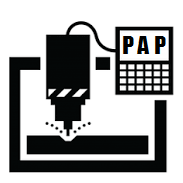
\includegraphics[scale=1.0]{Images/cnc_icon.png}}
%\author{CESE 2018 - FIUBA}

\institute{Director\\ Ing. Juan Manuel Cruz}
\date{Jurados\\ Esp. Ing. Eric Pernia\\
          Lic. Danilo Zechin\\
          Dr. Ing. Pablo Gómez
       }
%------------------------------------------------
\begin{document}

\begin{frame}
   \maketitle % Automatically created using the information in the commands above
   \begin{picture}(1,1)
      \put(240,280) {
         \hbox {
            
\includegraphics[trim=18mm  7mm  18mm 40mm,clip, width=0.3\textwidth]{./Figures/logo_fiuba.pdf}
         }
      }
   \end{picture}
\end{frame}


\begin{frame}{Motivación - Solución actual con PC}
   \begin{columns}
      \column{0.6\textwidth}
      \begin{center}
         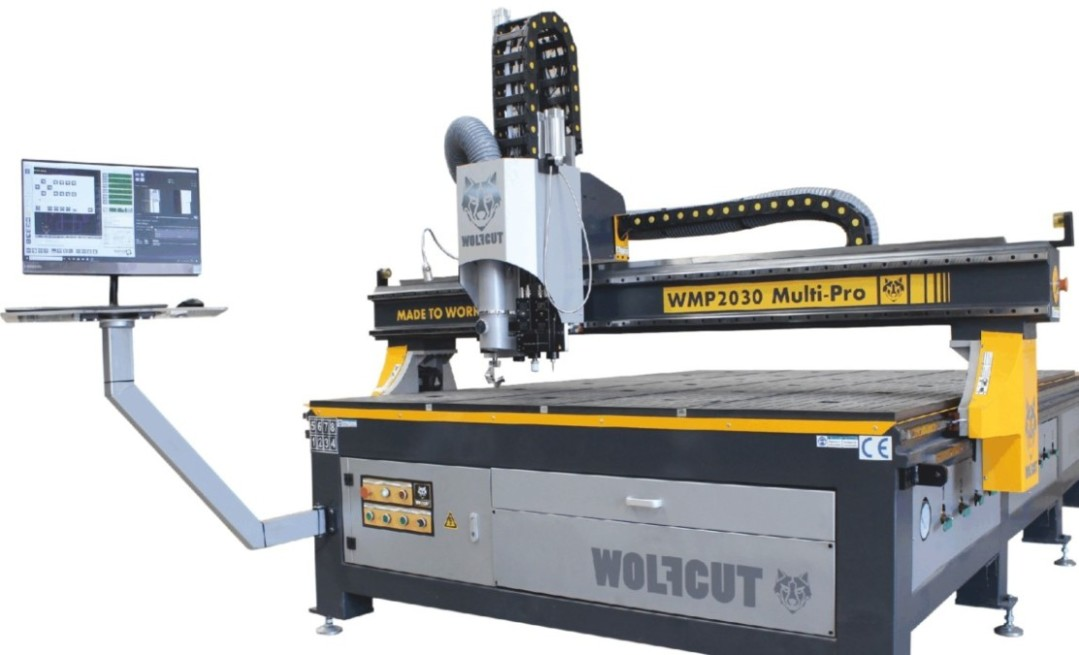
\includegraphics[width=\textwidth]{./Figures/wolfcut_cnc.jpg} \\
         \href{https://wolfcut.es/}{https://wolfcut.es/}
      \end{center}
      \column{0.4\textwidth}
      \begin{itemize}
         \item{Clientes de Diferentes industrias.}
      \begin{itemize}
         \item{Carton.}
         \item{Madera.}
         \item{Azulejos.}
         \item{Polifan.}
      \end{itemize}
         \item{PC.}
         \item{Interfaz.}
         \item{SO general.}
         \item{Software.}
         \item{Modificaciones.}
      \end{itemize}
   \end{columns}
\end{frame}
\begin{frame}{Motivación - Solución actual con PC}
   \begin{columns}
      \column{0.5\textwidth}
      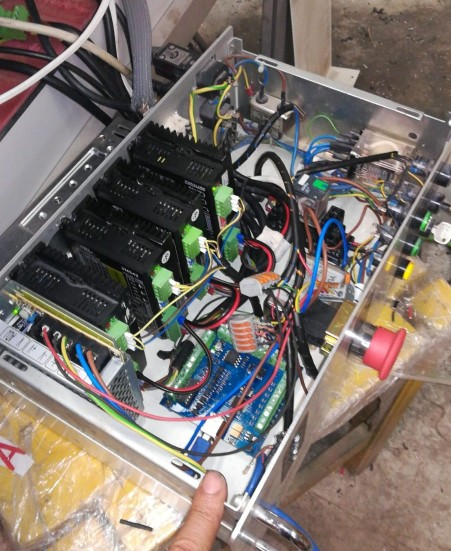
\includegraphics[width=\textwidth]{./Figures/tripas_wolfcut.jpg}
      \column{0.5\textwidth}
      Desventajas
      \begin{itemize}
         \item{Pulsos no uniformes.}
         \item{Baja confiabilidad.}
         \item{Software cerrado.}
         \item{Licencias costosas.}
         \item{Cableado complejo.}
         \item{Interfases poco apropiadas para uso industrial.}
         \item{No expansible.}
      \end{itemize}
   \end{columns}
\end{frame}

\begin{frame}{Motivación - Solución embebida}
   \begin{columns}
      \column{0.5\textwidth}
         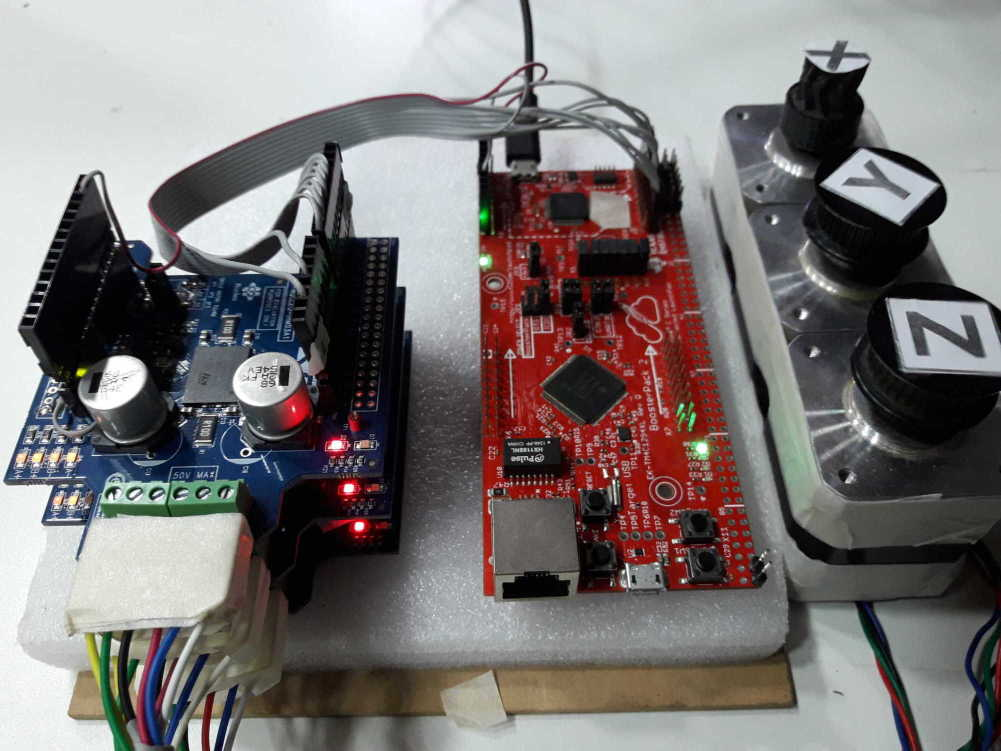
\includegraphics[width=\textwidth]{./Figures/prototipo_hardware4.jpg}
      \column{0.5\textwidth}
      Mejoras:
      \begin{itemize}
               \item{No requiere PC.}
               \item{Open Hard.}
               \item{Open Soft.}
               \item{Pulsos generados por hard.}
               \item{Acepta nuevos periféricos.}
      \end{itemize}
   \end{columns}
\end{frame}

\begin{frame}{Hardware - Driver de Motores de desarrollo}
   \begin{columns}
      \column{0.5\textwidth}
      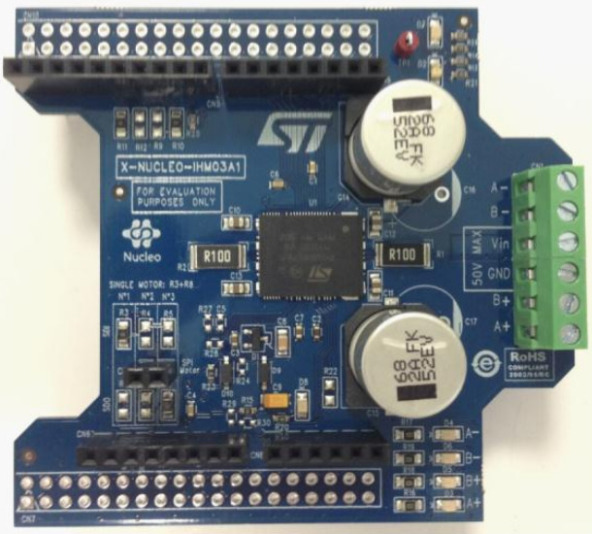
\includegraphics[width=\textwidth, left]{./Figures/xnucleo.jpg}
      \column{0.5\textwidth}
      Ventajas:
      \begin{itemize}
         \item{128 micropasos.}
         \item{Calibración por software.}
         \item{Control por SPI @ 5Mhz.}
      \end{itemize}
      Desventajas:
      \begin{itemize}
         \item{Tres drivers máximo.}
         \item{Diseñado en 4 layers.}
         \item{CLK no sincronizado.}
      \end{itemize}
   \end{columns}
\end{frame}

\begin{frame}{Hardware - Driver de Motores diseñado}
   \begin{columns}
      \column{0.5\textwidth}
      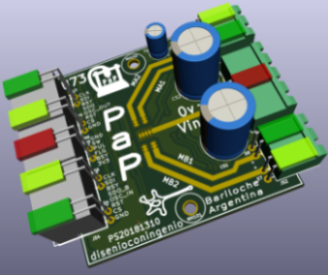
\includegraphics[width=\textwidth]{./Figures/kicad_top.png}
      \column{0.5\textwidth}
      Mejoras:
      \begin{itemize}
         \item{Sincronización de CLK.}
         \item{Sin máximo de drivers.}
         \item{Conectores enchufables.}
         \item{Apto montaje en gabinete.}
         \item{Diseñado en 2 layers.}
      \end{itemize}
   \end{columns}
\end{frame}

\begin{frame}{Hardware - PCB fabricado}
   \begin{columns}
      \column{0.5\textwidth}
      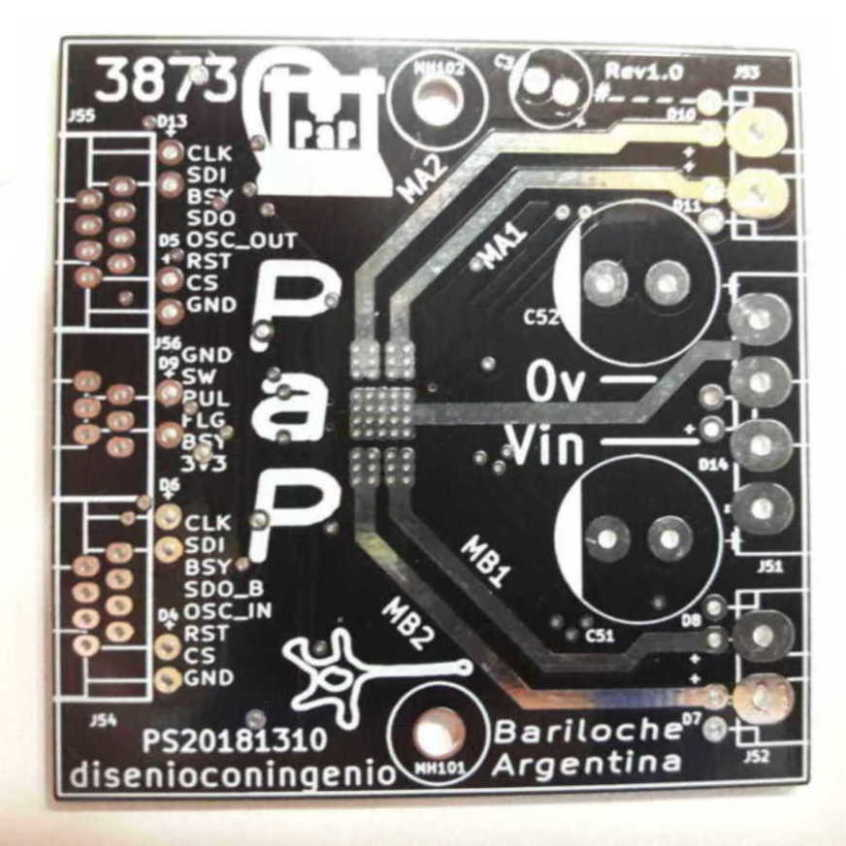
\includegraphics[width=\textwidth]{./Figures/proto_pap_top.jpg}
      \column{0.5\textwidth}
      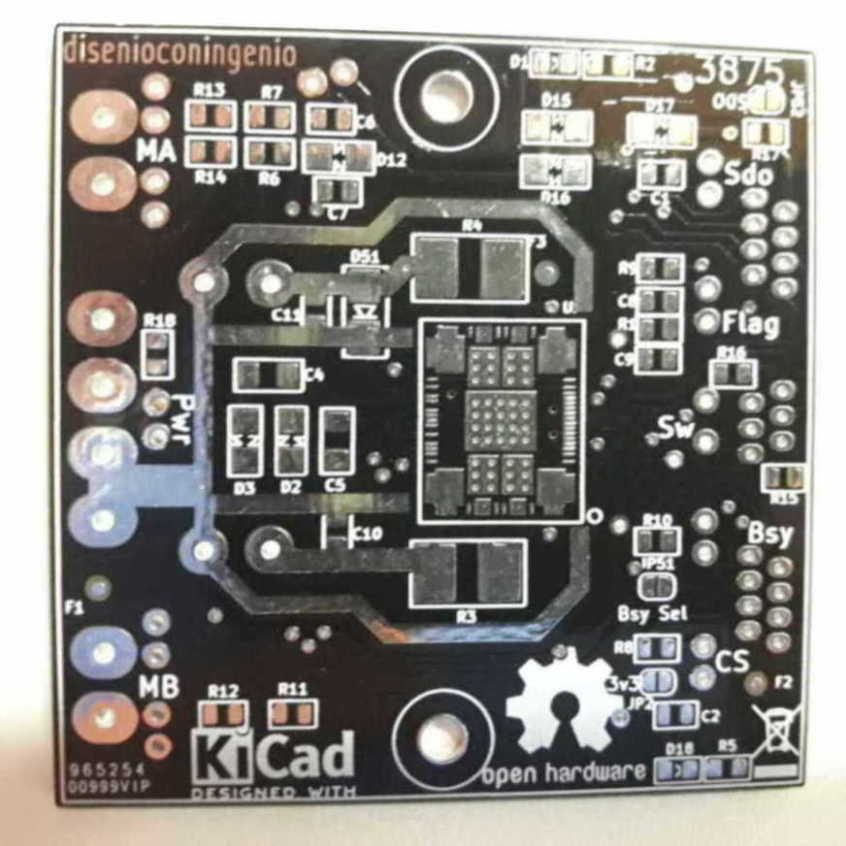
\includegraphics[width=\textwidth]{./Figures/proto_pap_bot.jpg}
   \end{columns}
\end{frame}

\begin{frame}{Hardware - Controlador utilizado}
   \begin{columns}
      \column{0.5\textwidth}
      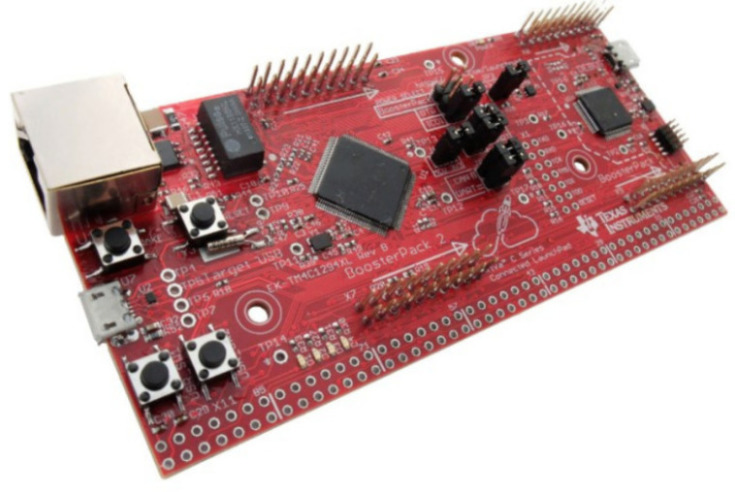
\includegraphics[width=\textwidth, right]{./Figures/tivac.jpg}
      \column{0.5\textwidth}
      \begin{itemize}
         \item{Cortex M4 @ 120Mhz.}
         \item{1MB flash /256KB RAM.}
         \item{Ethernet, SPI, UART, USB.}
         \item{Unidad de punto flotante.}
      \end{itemize}
   \end{columns}
\end{frame}

\begin{frame}{Hardware - Router de prueba - Video 1}
   \begin{columns}
      \column{0.5\textwidth}
   \href{run:./videos/video1.mp4}{
      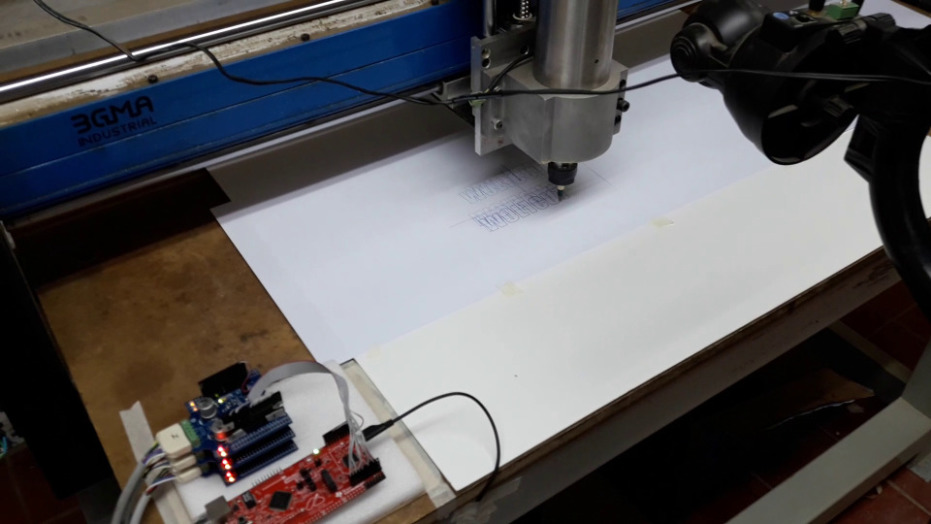
\includegraphics[width=\textwidth, left]{./videos/shot0001.jpg}
   }
   \href{https://youtu.be/09bBvzOHA3k}{https://youtu.be/09bBvzOHA3k}
      \column{0.5\textwidth}
      Se muestra:
      \begin{itemize}
         \item{Router típico modificado.}
         \item{Conexiones entre router y prototipo.}
         \item{Trazador adaptado a husillo.}
      \end{itemize}
   \end{columns}
\end{frame}


\begin{frame}{Firmware - Introducción a Gcode}
   \begin{columns}
      \column{0.5\textwidth}
      \begin{itemize}
         \item{Norma NIST RS274NGC V3 2000.}
         \item{Archivo de texto.}
         \item{Entrada manual.}
         \item{Variantes segun el fabricante.}
         \item{TDD y Ceedling para el intérprete.}
      \end{itemize}

      \column{0.5\textwidth}
      Ejemplo de un archivo GCode:
      \begin{itemize}
         \item{N1 G1 X10}
         \item{N2 G1 X-0.45 Z0020.12300}
         \item{N3 G1 Y002.02 Z100. F600}
      \end{itemize}
   \end{columns}
\end{frame}


\begin{frame}[fragile]{Firmware - Estrategia de movimientos GCode}
   \begin{columns}
      \column{0.5\textwidth}
      \begin{itemize}
         \item{Parada exacta:}
            \begin{itemize}
               \item{Esquinas marcadas.}
               \item{Movimientos lentos.}
               \item{Cortes geométricos.}
            \end{itemize}
         \item{Camino exacto.}
            \begin{itemize}
               \item{Cambia la velocidad para preservar el camino.}
               \item{Puede detenerse.}
               \item{Geometría con curvas.}
               \item{Compromiso entre velocidad y precisión.}
            \end{itemize}
         \item{Modo continuo.}
            \begin{itemize}
               \item{Redondea las esquinas.}
               \item{Intenta preservar la velocidad.}
               \item{Trabajos rápidos pero de baja precisión.}
            \end{itemize}
      \end{itemize}
      \column{0.5\textwidth}
      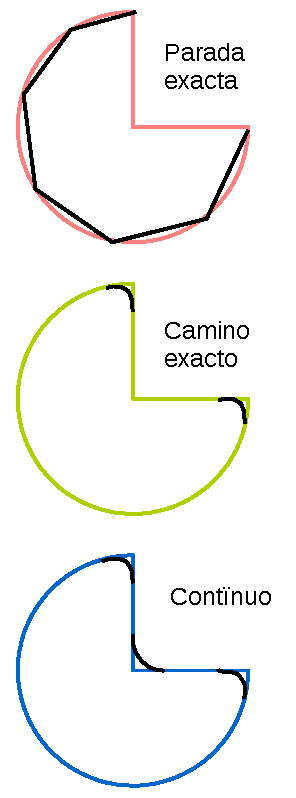
\includegraphics[width=0.5\textwidth, left]{./Figures/exact_stop.pdf}
   \end{columns}
\end{frame}

\begin{frame}[fragile]{Firmware - Cálculos de movimiento de GCode}
   \begin{columns}
      \column{0.3\textwidth}
      \begin{lstlisting}
GCode:
---------------
N1 G1 X0 Y0
N2 X4 Y3
---------------
      \end{lstlisting}
Ecuaciones:
      \begin{align}
         \notag
         d   &= \sqrt{d_x^2 + d_Y^2} \\
         \notag 
         X   &= V_0 t + \frac{1}{2} a t^2 \\
         \notag 
         t_f &= \frac{V_f}{a} \\
         \notag 
         X_f &= \frac{V_f^2}{2a}
      \end{align}
      \begin{lstlisting}
---------------
      \end{lstlisting}
      \column{0.7\textwidth}
      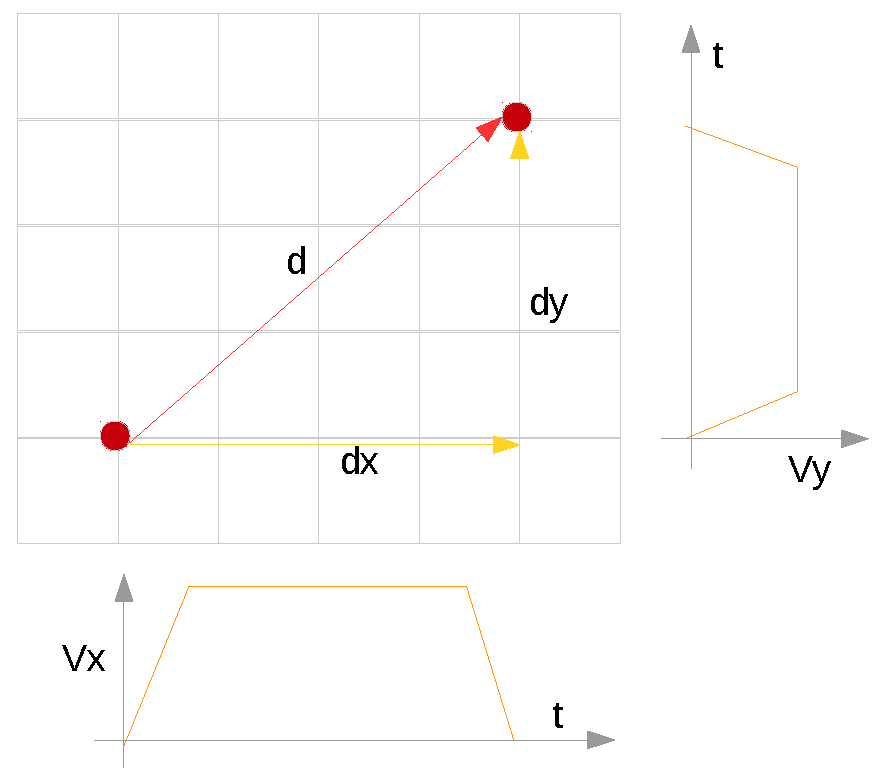
\includegraphics[width=\textwidth, left]{./Figures/gcode.pdf}
   \end{columns}
\end{frame}

\begin{frame}[fragile]{Firmware - Cálculos de movimiento de GCode}
   \begin{columns}
      \column{0.3\textwidth}
\begin{align}
   \notag
   t_a   &= \frac{V_f}{a} \\
   \notag
   \\
   \notag
   X_a   &= \frac{V_f^2}{2a} \\
   \notag
   X_d   &= \frac{V_f^2}{2d} \\
   \notag
   X_c   &= X-X_a-X_d \\
   \notag
   \\
   \notag
   t_c   &= \frac{V_f}{X_c}
   \notag
\end{align}
\boxed{Timer = t_a+t_c}
      \column{0.7\textwidth}
      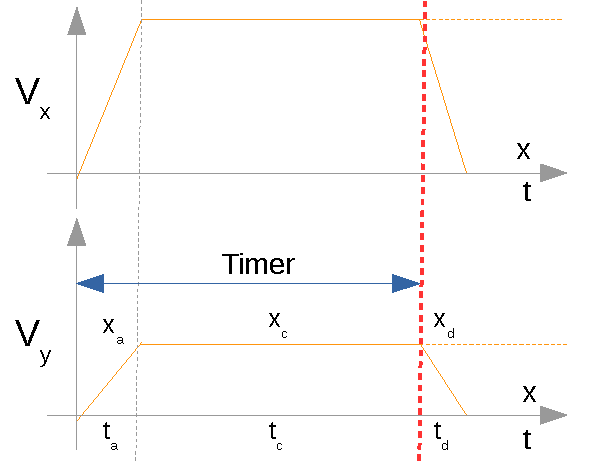
\includegraphics[width=\textwidth, left]{./Figures/gcode2.pdf}
   \end{columns}
\end{frame}

%\begin{frame}{Firmware - Esquema temporal}
%   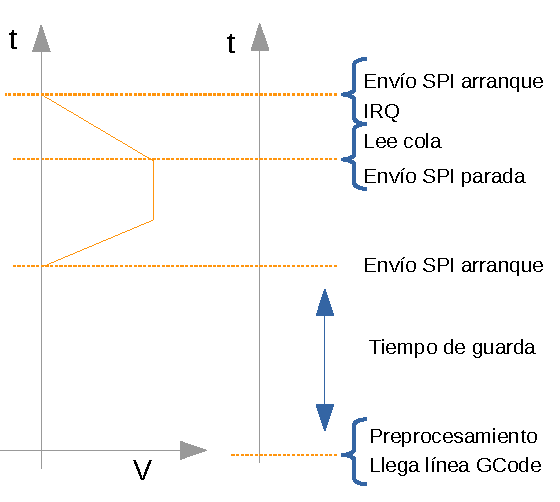
\includegraphics[width=0.8\textwidth, center]{./Figures/buffer.pdf}
%\end{frame}

\begin{frame}{Firmware - Diagrama de flujo}
   \begin{columns}
      \column{0.5\textwidth}
   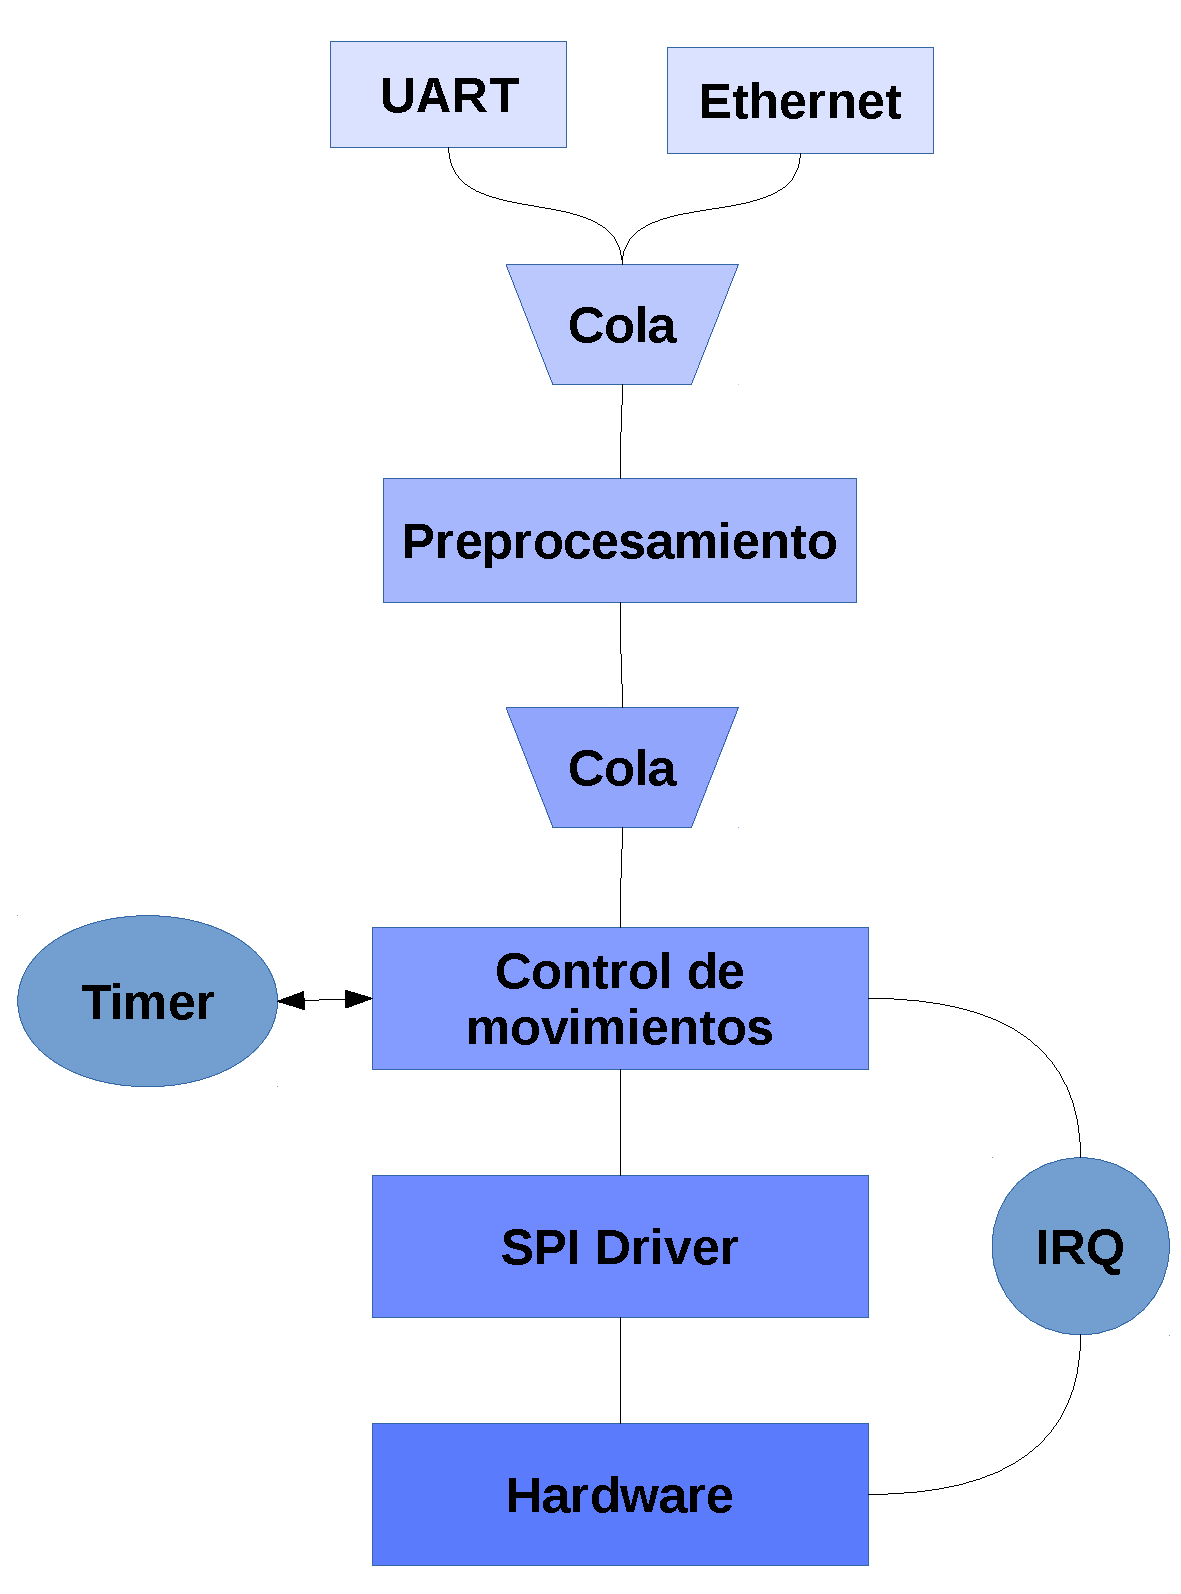
\includegraphics[width=\textwidth]{./Figures/firmware_flujo_basico.pdf}
      \column{0.5\textwidth}
      \begin{itemize}
         \item{FreeRTOS.}
         \item{Colas.}
         \item{Mutex.}
         \item{Semáforos.}
         \item{lwIP.}
         \item{Telnet.}
         \item{Terminal de comandos.}
         \item{GPIO IRQ.}
         \item{Raíz cuadrada.}
         \item{Operaciones de punto flotante.}
      \end{itemize}
   \end{columns}
\end{frame}

\begin{frame}{Firmware - Control manual - Video 2}
   \begin{columns}
      \column{0.5\textwidth}
   \href{run:./videos/video2.mp4}{
      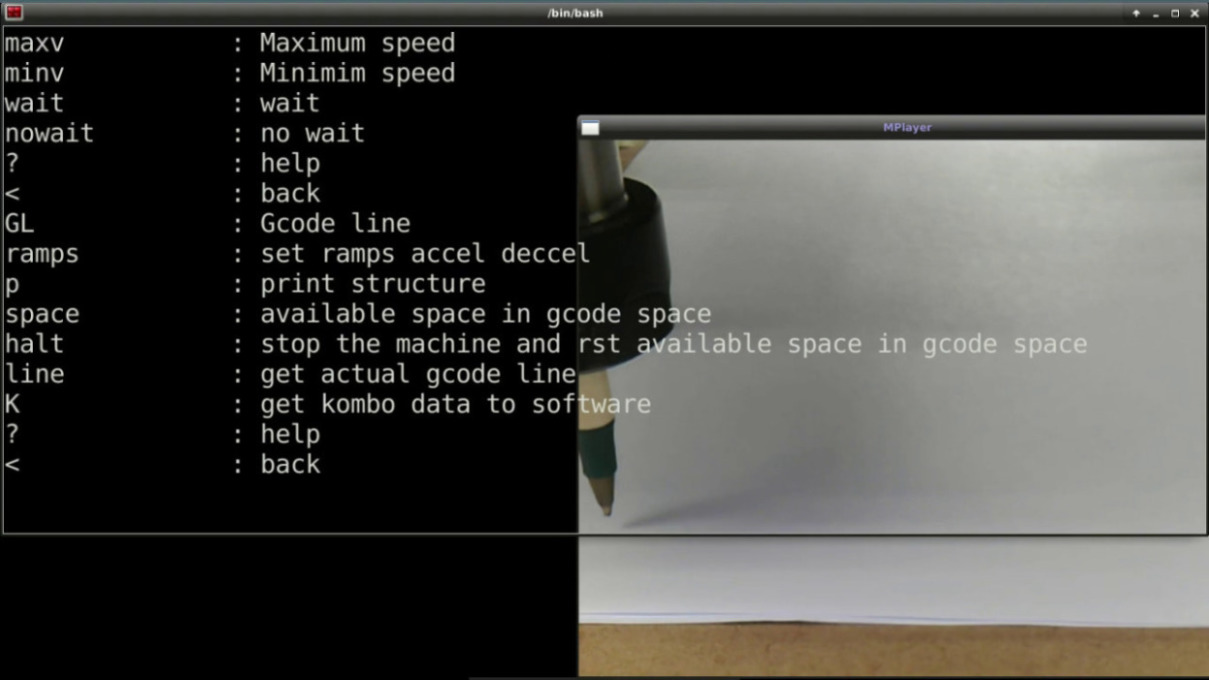
\includegraphics[width=\textwidth, left]{./videos/shot0002.jpg}
   }
   \href{https://youtu.be/nLbHyZ5A89Q}{https://youtu.be/nLbHyZ5A89Q}
      \column{0.5\textwidth}
      Se muestra:
      \begin{itemize}
         \item{Conexión manual al router.}
         \item{Acceso por ethernet y serie.}
         \item{Envío de GCode manual.}
      \end{itemize}
   \end{columns}
\end{frame}

\begin{frame}{Software - Ejecutando un trazado - Video 3}
   \begin{columns}
      \column{0.5\textwidth}
   \href{run:./videos/video3.mp4}{
      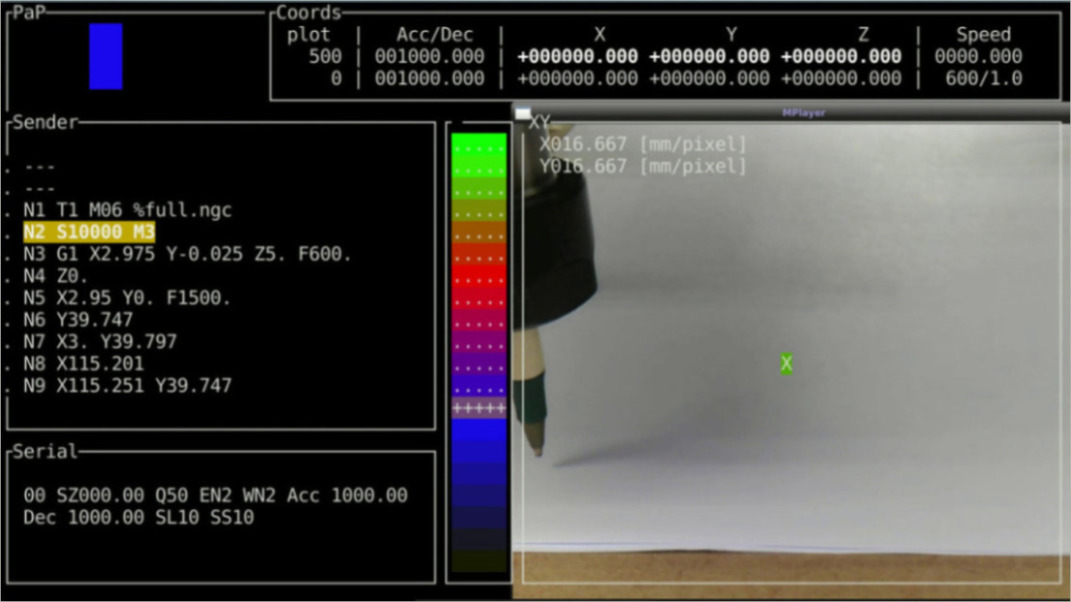
\includegraphics[width=\textwidth, left]{./videos/shot0003.jpg}
   }
   \href{https://youtu.be/3zYNtZtnbnQ}{https://youtu.be/3zYNtZtnbnQ}
      \column{0.5\textwidth}
      Se muestra:
      \begin{itemize}
         \item{Envió de archivos Gcode.}
         \item{Cambio de aceleración.}
         \item{Cambio de velocidad.}
         \item{Jog manual.}
         \item{Visualización del recorrido.}
         \item{Visualización de buffer.}
         \item{Acceso desde ssh/telnet.}
      \end{itemize}
   \end{columns}
\end{frame}


\begin{frame}{Conclusión: Trabajo en Madera - Video 4}
   \begin{columns}
      \column{0.5\textwidth}
   \href{run:./videos/video4.mp4}{
      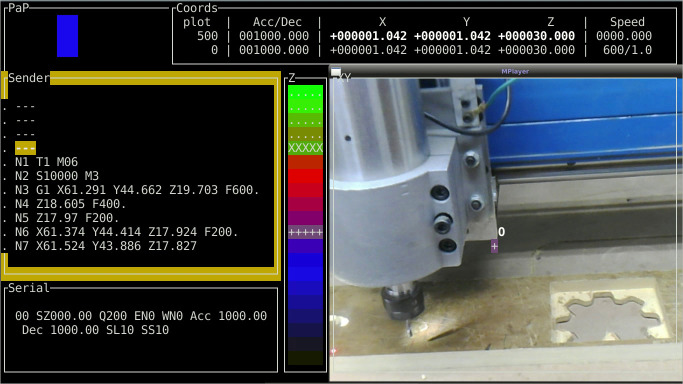
\includegraphics[width=\textwidth, left]{./videos/shot0004.jpg}
   }
   \href{https://youtu.be/Y-lOf3UwYmc}{https://youtu.be/Y-lOf3UwYmc}

      \column{0.5\textwidth}
      Se muestra:
      \begin{itemize}
         \item{Maquinado en madera.}
         \item{1h:30m de trabajo.}
         \item{Maquinado de esfera, recorrido geometrico y agujereado.}
      \end{itemize}
   \end{columns}
\end{frame}

\begin{frame}{Conclusiones - Piezas en madera y trazados}
      
\includegraphics[width=\textwidth]{./Figures/ciaa_en_madera.jpg}
\end{frame}

\begin{frame}{Conclusiones}
   \begin{columns}
      \column{0.5\textwidth}
      \begin{itemize}
         \item{Driver completo del powerstep01}
         \item{PCB de potencia.}
         \item{Software de control.}
      \end{itemize}
      \column{0.5\textwidth}
      \begin{itemize}
         \item{Modo camino exacto.}
         \item{Conexion ethernet y serial.}
         \item{Codigo parametrizado para mas motores.}
         \item{Mecanizado de piezas.}
      \end{itemize}
   \end{columns}
\end{frame}

\begin{frame}{Próximos pasos}
   \begin{columns}
      \column{0.5\textwidth}
      \begin{itemize}
         \item{Camino exacto.}
         \item{Modo continuo.}
         \item{Software por red.}
         \item{Almacenamiento interno.}
         \item{Completar intérprete de GCode.}
      \end{itemize}
      \column{0.5\textwidth}
      \begin{itemize}
         \item{Optimización de cálculos.}
         \item{Optimización lazo de control.}
         \item{Validacion de PCB fabricado.}
         \item{Fines de carrera.}
         \item{Control de husillo.}
      \end{itemize}
   \end{columns}
\end{frame}
%%------------------------------------------------
%
\begin{frame}{Preguntas?}
      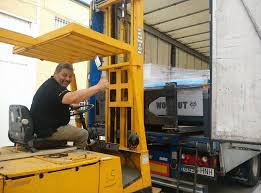
\includegraphics[width=\textwidth]{./Figures/sanchez.jpg}
\end{frame}

%----------------------------------------------------------------------------------------
%   CLOSING/SUPPLEMENTARY SLIDES
%----------------------------------------------------------------------------------------

\appendix
%
\begin{frame}{References}
   \nocite{*} % Display all references regardless of if they were cited
   \bibliography{example.bib}
   \bibliographystyle{plain}
\end{frame}

\end{document}
